\chapter{Lec 14 - Dealing with Uncertainty}
\section{Uncertainty}
Agents may need to handle \textbf{uncertainty}, whether due to partial observability, nondeterminism, or a combination of the two. Suppose, for example, that an automated taxi has the goal of delivering a passenger to the airport on time. The agent forms a plan, $A_{90}$, that involves leaving home 90
minutes before the flight departs and driving at a reasonable speed. Even though the airport is only about 5 miles away, a logical taxi agent will not be able to conclude with certainty that “Plan $A_{90}$ will get us to the airport in time.” Instead, it reaches the weaker conclusion “Plan $A_{90}$ will get us to the airport in time, as long as the car doesn’t break down or run out of gas, and I don’t get into an accident, and there are no accidents on the bridge, and the plane doesn’t leave early, and no meteorite hits the car, and ... .”  None of these conditions can be deduced for sure, so the plan’s success cannot be inferred. Other plans, such as $A_{180}$, might increase the agent’s belief that it will get to the airport on
time, but also increase the likelihood of a long wait. \textit{The right thing to do, the rational decision, therefore depends on both the relative importance of various goals and the likelihood that, and degree to which, they will be achieved.}
\newline\newline
A logical agent believes each sentence to be true or false or has no opinion, whereas a probabilistic agent may have a numerical degree of belief between 0 (for sentences that are certainly false) and 1 (certainly true). \textbf{Probability} provides a way of summarizing the uncertainty that comes from our
\begin{itemize}
    \item \textbf{laziness:}  failure to enumerate exceptions, qualifications, etc.
    \item \textbf{ignorance}: lack of relevant facts, initial conditions, etc.
\end{itemize}
Probabilities relate propositions to one’s own state of knowledge, e.g. $P(A_{25}|\,\, \text{no reported accidents}) = 0.06$. These are not claims of some probabilistic tendency in the current situation, but might be learned from past experience of similar situations. Probabilities of propositions change with new evidence: 
\[P(A_{25}|\,\, \text{no reported accidents, 5 a.m.}) = 0.15\]
Consider again the $A_{90}$ plan for getting to the airport. Suppose it gives us a 97\% chance of catching our flight. Does this mean it is a rational choice? Not necessarily: there might be other plans, such as $A_{180}$, with higher probabilities.  If it is vital not to miss the flight, then it is worth risking the longer wait at the airport. What about $A_{1440}$, a plan that involves
leaving home 24 hours in advance? In most circumstances, this is not a good choice, because although it almost guarantees getting there on time, it involves an intolerable wait.\\\\
To make such choices, an agent must first have \textbf{preferences} between the different possible outcomes of the various plans. We use \textbf{utility theory} to represent and reason with preferences.  Utility theory says that every state has a degree of usefulness, or utility, to an agent and that the agent will prefer states with higher utility. Preferences, as expressed by utilities, are combined with probabilities in the general theory of rational decisions called \textbf{decision theory}:
\[\textit{Decision theory} = \textit{Probability theory} + \textit{Utility theory}\]

\section{Probability notation}
For our agent to represent and use probabilistic information, we need a formal language.
\begin{itemize}
    \item Probabilities such as $P(Cavity = true)=0.1$ and $P(Weather = sunny)=0.72$ are called \textbf{prior} or \textbf{unconditional} probabilities. They refer to degrees of belief in propositions in the absence of any other information.

    \item Most of the time, we have some information, usually called \textbf{evidence}, that has already been revealed. In this case we have the \textbf{conditional} or \textbf{posterior} probability. For example, $P(cavity|toothache)=0.6$. This assertion does \textbf{not} mean “Whenever toothache is true, conclude that cavity is true with probability 0.6”. Rather it means “Whenever toothache is true and we have no further information, conclude that cavity is true with probability 0.6.”  The extra condition is important; for example, if we had the further information that the dentist found no cavities, we definitely would not want to conclude that cavity is true with probability 0.6; instead we need to use $P(cavity|toothache \land \neg cavity)=0.$ Note also that new evidence may be irrelevant, allowing simplification, e.g., $P(cavity|toothache, InterWin) = P(cavity|toothache)=0.6$.\\\\
    Mathematically speaking, conditional probabilities are defined in terms of unconditional probabilities as follows: for any events $a$ and $b$, we have
    \[P(a | b) = \frac{P(a \land b)}{P(b)}\]
    The definition of conditional probability  can be written in a different form called the \textbf{product rule}:
    \[P(a \land b) = P(a|b)P(b)\]
    
    
    
    \item Variables in probability theory are called \textbf{random variables} and their names begin with an uppercase letter. Every random variable has a \textbf{domain}, the set of possible values it can take on. A \textbf{Probability distribution} gives values for all possible assignments to a random variable. E.g., if $Weather$ can take values in \\$<sunny,rain,cloudy,snow>$, then
    \[\textbf{P}(Weather) = <0.72, 0.1, 0.08, 0.1>\]
     Normalized, i.e., sums to 1. For continuous variables, it is not possible to write out the entire distribution as a vector, because there are infinitely many values. Instead, we can define the probability that a random variable takes on some value $x$ as a parameterized function of $x$. We call this a \textbf{probability density function}.

     \item In addition to distributions on single variables, we need notation for distributions on multiple variables. The \textbf{Joint probability distribution} for a set of random variables gives the probabilities of all combinations of the values of those random variables (i.e., every sample point). For example, $\textbf{P}(Weather, Cavity)$ is a $4 \times 2$ table of probabilities:
     \begin{center}
         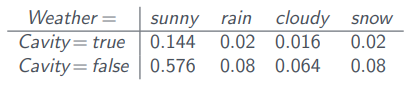
\includegraphics[]{images/joint-prob.png}
     \end{center}
     Every question about a domain can be answered by the joint distribution because every event is a sum of sample points.\\\\
     Any joint probability distribution over many random variables may be decomposed into conditional distributions.
     \begin{center}
         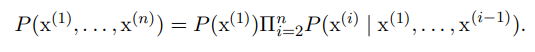
\includegraphics[]{images/chain-rule.png}
     \end{center}
     This observation is known as the \textbf{chain rule} of probability.
\end{itemize}

\section{Inference by enumeration}
Inference by enumeration means doing inference using only full joint distributions. \textbf{Probabilistic inference} is the computation of posterior probabilities for query propositions given observed evidence.\\\\
We begin with a simple example: a domain consisting of just the three Boolean variables $Toothache$, $Cavity$, and $Catch$ (the dentist’s nasty steel probe catches in my tooth). The full joint distribution is a $2 \times 2 \times 2$ table.
\begin{center}
    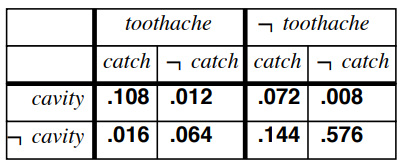
\includegraphics[]{images/dentist-table.png}
\end{center}
The probability associated with a proposition is defined to be the sum of the probabilities of the atomic events in which it holds: For any proposition $\phi$
\[P(\phi) = \sum_{w \in \phi}P(w)\]
For example, when rolling fair dice, we have $P(Total = 11) = P((5, 6)) + P((6, 5)) = 1/36 + 1/36 = 1/18$. \\\\
Then, we can calculate the probability $P(cavity \lor toothache)$ as follows:
\[P(cavity \lor toothache) = 0.108 + 0.012 + 0.072 + 0.008 + 0.016 + 0.064 = 0.28\]
We  simply identify those events in which the proposition is true and add up their probabilities.
\begin{center}
    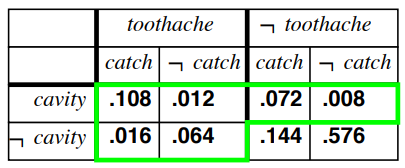
\includegraphics[]{images/dentist-table-2.png}
\end{center}
One particularly common task is to extract the distribution over some subset of variables or a single variable. For example, adding the entries in the first row gives the unconditional or \textbf{marginal probability} of cavity:
\[P(cavity) = 0.108 + 0.012 + 0.072 + 0.008 = 0.2\]
This process is called \textbf{marginalization}, or \textbf{summing out}, because we sum up the probabilities for each possible value of the other variables. We can write the following general marginalization rule for any sets of variables $\textbf{Y}$ and $\textbf{Z}$:
\[\textbf{P}(\textbf{Y}) = \sum_{\textbf{z} \in \textbf{Z}}\textbf{P}(\textbf{Y}, \textbf{z})\]
where $\sum_{\textbf{z} \in \textbf{Z}}$ means to sum over all the possible combinations of values of the set of variables $\textbf{Z}$.
\[\textbf{P}(Cavity) = \sum_{\textbf{z} \in \{Catch, Toothache\}} \textbf{P}(Cavity, \textbf{z})\]
We can also compute conditional probabilities, for example:
\[
\begin{split}
    P(cavity | toothache) & = \frac{P(cavity \land toothache)}{P(toothache)}\\
    & = \frac{0.108 + 0.012}{0.108 + 0.012 + 0.016 + 0.064}\\
    & = 0.6
\end{split}
\]
Just to check, we can also compute the probability that there is no cavity, given a toothache:
\[
\begin{split}
    P(\neg cavity | toothache) & = \frac{P(\neg cavity \land toothache)}{P(toothache)}\\
    & = \frac{0.016 + 0.064}{0.108 + 0.012 + 0.016 + 0.064}\\
    & = 0.4
\end{split}
\]
The two values sum to 1.0, as they should. Notice that in these two calculations the term $1/P(toothache )$ remains constant, no matter which value of $Cavity$ we calculate. In fact, it can be viewed as a normalization constant for the distribution $\textbf{P}(Cavity |toothache)$, ensuring that it adds up to 1. With this notation, we can write the two preceding equations in one:
\begin{center}
    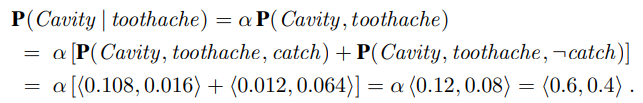
\includegraphics[]{images/prob-inference-rule.png}
\end{center}
Where $\alpha$ is the normalization constant. In other words, we can calculate $\textbf{P}(Cavity |toothache)$ even if we don’t know the value of $P(toothache)$. We temporarily forget about the factor $1/P(toothache )$ and add up the values for $cavity$ and $\neg cavity$, getting 0.12 and 0.08. Those are the correct relative proportions, but
they don’t sum to 1, so we normalize them by dividing each one by 0.12 + 0.08, getting the true probabilities of 0.6 and 0.4.\\\\
From the example, we can extract a general inference procedure. We begin with the case in which the query involves a single variable, $X$ (Cavity in the example).  Let $\textbf{E}$ be the list of evidence variables (just $Toothache$ in the example), let $\textbf{e}$ be the list of observed values for them,  and let $\textbf{Y}$ be the remaining unobserved (hidden) variables (just $Catch$ in the example). The query is $\textbf{P}(X | \textbf{e})$ and can be evaluated as:
\[\textbf{P}(X | \textbf{e}) = \alpha \textbf{P}(X, \textbf{e}) = \alpha \sum_{\textbf{y}}\textbf{P}(X, \textbf{e}, \textbf{y})\]
where the summation is over all possible $\textbf{y}$s (i.e., all possible combinations of values of the unobserved variables $\textbf{Y}$).\\\\
Given the full joint distribution to work with, this inference procedure can answer probabilistic
queries for discrete variables. It does not scale well, however: for a domain described by $n$ Boolean variables, it requires an input table of size $O(2^n)$ and takes $O(2^n)$ time to process the table.

\section{Independence}
Two variables $X$ and $Y$ are \textbf{independent} iff
\[\textbf{P}(X | Y ) = \textbf{P}(X)\,\, \text{or} \,\,\textbf{P}(Y | X) = \textbf{P}(Y)\,\, \text{or}\,\, \textbf{P}(X, Y ) = \textbf{P}(X)\textbf{P}(Y )\]
Let us expand the full joint distribution seen before by adding a fourth variable, $Weather$. The full joint distribution then becomes $\textbf{P}(Toothache, Catch, Cavity,Weather )$, which has $2 \times 2 \times 2 \times 4 = 32$ entries. We may ask how these variables are related, for example, how are $P(toothache, catch, cavity, cloudy)$
and $P(toothache, catch, cavity)$ related? We can use the product rule:
\[P(toothache, catch, cavity, cloudy)
= P(cloudy |toothache, catch, cavity)P(toothache, catch, cavity)\]
Now, it seems safe to say that the weather does not influence the dental variables. Therefore, the following assertion seems reasonable:
\[P(cloudy |toothache, catch, cavity) = P(cloudy)\]
From this, we can deduce:
\[P(toothache, catch, cavity, cloudy) = P(cloudy)P(toothache, catch, cavity)\]
A similar equation exists for every entry in $\textbf{P}(Toothache, Catch, Cavity,Weather)$. In fact, we can write the general equation:
\[\textbf{P}(Toothache, Catch, Cavity, Weather ) = \textbf{P}(Toothache, Catch, Cavity)\textbf{P}(Weather ) .\]
Therefore, the weather is independent of one’s dental problems.\\\\
If the complete set of variables can be divided into independent subsets, then the full joint distribution can be \textbf{factored} into separate joint distributions on those subsets. In a more practical vein, the independence of
dentistry and meteorology is a good thing, because otherwise the practice of dentistry might require intimate knowledge of meteorology, and vice versa. When they are available, then, independence assertions can help in reducing the size of
the domain representation and the complexity of the inference problem. Unfortunately, clean separation of entire sets of variables by independence is quite rare.

